\documentclass{article}
\usepackage{amsmath}
\usepackage{hyperref}
\usepackage{tikz}
\usetikzlibrary{calc,arrows,shapes,positioning,automata}
\usepackage{tkz-euclide}
\usepackage[numbib]{tocbibind}
\usepackage{float}
\usepackage{array}
\usepackage{bm}
\usepackage{siunitx}  
\usepackage{xstring}
\usepackage{catchfile}

\CatchFileDef{\headfull}{../.git/HEAD}{}
\StrGobbleRight{\headfull}{1}[\head]
\StrBehind[2]{\head}{/}[\branch]
\IfFileExists{../.git/refs/heads/\branch}{%
    \CatchFileDef{\commit}{../.git/refs/heads/\branch}{}}{%
    \newcommand{\commit}{\dots~(in \emph{packed-refs})}}
\newcommand{\gitrevision}{%
  \StrLeft{\commit}{7}%
}

\begin{document}

% Tikz code used to support block diagrams
% credit: https://tex.stackexchange.com/questions/175969/block-diagrams-using-tikz

\tikzset{
block/.style = {draw, fill=white, rectangle, minimum height=3em, minimum width=3em},
tmp/.style  = {coordinate}, 
circ/.style= {draw, fill=white, circle, node distance=1cm, minimum size=0.6cm},
input/.style = {coordinate},
output/.style= {coordinate},
pinstyle/.style = {pin edge={to-,thin,black}}
}

\title{FreeDV-060 Radio Autoencoder (RADE) V2 Test Report}
\author{David Rowe VK5DGR}
\date{\today \quad Git: \texttt{\gitrevision} on branch \texttt{\branch}\\}
\maketitle

\section{Introduction}

This document describes the tests performed on the prototype RADE V2 waveform, and the test results.

\subsection{Acknowledgements}

The RADE concept evolved from a discussion between Jean-Marc Valin and David Rowe, after which Jean-Marc quickly put together an initial proof-of-concept demo. Over a period of several months David built on this work to develop a practical over the air waveform for speech over HF radio channels. This waveform is denoted RADE V1. 
Over the course of 2025 and early 2026 David worked on developing RADEV2, which has several novel innovations:
\begin{itemize}
\item Using ML to handle HF channel phase distortion, fine frequency offsets, and small timing estimates.
\item No pilot or unique word symbols.
\item A $N_c=14$ waveform with a 800 \si{Hz} 99\% occupied bandwidth (OBW).
\item PAPR set by a filter inside the encoder.
\item Low latency frame of around 40 \si{ms}.
\item ML based frame sync, rather than pilot symbols.
\end{itemize}
Jean-Marc again assisted with suggestion for timing estimation and frequency offset estimation.

The FreeDV Project Leadership Team and many others have helped with support and testing. The contributions from David, Mooneer and the FreeDV PLT was generously supported by a grant from Amateur Radio Digital Communications (ARDC).

\section{Feb 2026 Test Results}

\subsection{configuration}

\begin{table} [h]
\caption{Configuration for test campaign.}
\label{tab:time_to_acq}
\centering
\begin{tabular}{ l | l }
 \hline
  Date  & From 5 Feb 2026 \\
  Git Hash & bda6f2 \\
  ML encoder/decoder & 250725 \\
  ML sync & 250725a\_ml\_sync \\
 \hline
\end{tabular}
\end{table}

\subsection{Overall Performance}

The script \emph{./compare\_models\_inf.sh -p 260203\_inf} was used to generate loss versus SNR/PNR curves (plotted in Figure \ref{fig:260203_inf_loss_SNR3k_models}) for the following conditions:
\begin{itemize}
\item RADE V1 AWGN and MPP channels.
\item RADE V2 with no timing estimator, state machine, of frequency offset estimator (Genie V2) using \emph{inference.sh}.
\item RADE V2 with real world estimators and state machine using \emph{rx2.sh}.
\end{itemize}

The RADE V1 simulation is run using the \emph{inference.sh} script with phase equalisation but without timing estimation.  Spot checks of RADE V1 indicate this has no measurable affect on loss versus SNR.  The V2 curves with and without estimators are coincident, showing the estimator algorithms have a small impact on performance.  The high SNR on the green V2 curve at less than -1 \si{dB} is a measurement artefact due to the state machine falling out of sync at low SNRs; decoded audio is still possible as it recovers and re-syncs.
Looking at the AWGN curves on the loss versus SNR plot, for any SNR above 5 \si{dB}, the loss of V2 is less than V1.
The performance target for V2 was 3 \si{dB} over V1. Taking into account the PAPR gains (loss versus PNR curve), gains over V1 of approximately 3 \si{dB} can be observed at low PNRs on the MPP curves.

\begin{figure}[h]
\caption{Loss versus SNR and PNR for various RADE V1, and RADE V2 with and without estimators.}
\label{fig:260203_inf_loss_SNR3k_models}
\begin{center}
\scalebox{.9}{% Title: gl2ps_renderer figure
% Creator: GL2PS 1.4.2, (C) 1999-2020 C. Geuzaine
% For: Octave
% CreationDate: Sat Feb  7 11:46:16 2026
\setlength{\unitlength}{1pt}
\begin{picture}(0,0)
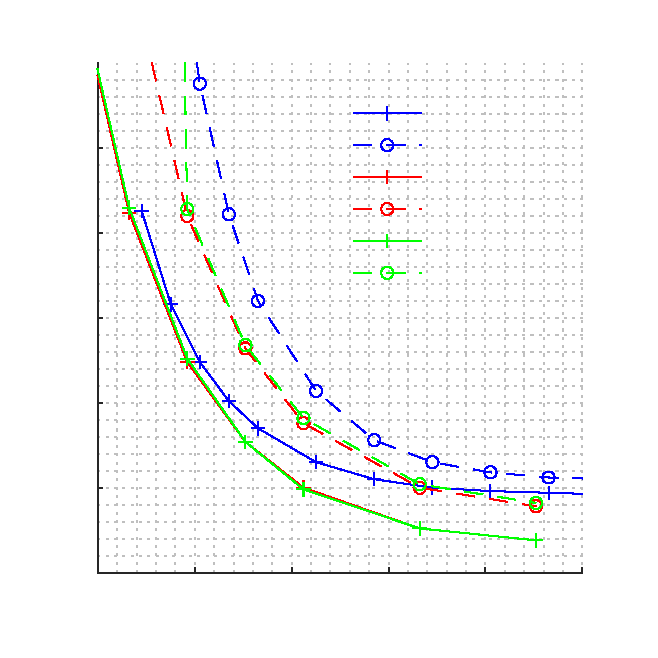
\includegraphics[scale=1]{260203_inf_loss_SNR3k_models-inc}
\end{picture}%
\begin{picture}(300,300)(0,0)
\fontsize{6}{0}\selectfont\put(39,28.228){\makebox(0,0)[t]{\textcolor[rgb]{0.15,0.15,0.15}{{-5}}}}
\fontsize{6}{0}\selectfont\put(85.5,28.228){\makebox(0,0)[t]{\textcolor[rgb]{0.15,0.15,0.15}{{0}}}}
\fontsize{6}{0}\selectfont\put(132,28.228){\makebox(0,0)[t]{\textcolor[rgb]{0.15,0.15,0.15}{{5}}}}
\fontsize{6}{0}\selectfont\put(178.5,28.228){\makebox(0,0)[t]{\textcolor[rgb]{0.15,0.15,0.15}{{10}}}}
\fontsize{6}{0}\selectfont\put(225,28.228){\makebox(0,0)[t]{\textcolor[rgb]{0.15,0.15,0.15}{{15}}}}
\fontsize{6}{0}\selectfont\put(271.5,28.228){\makebox(0,0)[t]{\textcolor[rgb]{0.15,0.15,0.15}{{20}}}}
\fontsize{6}{0}\selectfont\put(35.832,33){\makebox(0,0)[r]{\textcolor[rgb]{0.15,0.15,0.15}{{0.05}}}}
\fontsize{6}{0}\selectfont\put(35.832,73.75){\makebox(0,0)[r]{\textcolor[rgb]{0.15,0.15,0.15}{{0.1}}}}
\fontsize{6}{0}\selectfont\put(35.832,114.5){\makebox(0,0)[r]{\textcolor[rgb]{0.15,0.15,0.15}{{0.15}}}}
\fontsize{6}{0}\selectfont\put(35.832,155.25){\makebox(0,0)[r]{\textcolor[rgb]{0.15,0.15,0.15}{{0.2}}}}
\fontsize{6}{0}\selectfont\put(35.832,196){\makebox(0,0)[r]{\textcolor[rgb]{0.15,0.15,0.15}{{0.25}}}}
\fontsize{6}{0}\selectfont\put(35.832,236.75){\makebox(0,0)[r]{\textcolor[rgb]{0.15,0.15,0.15}{{0.3}}}}
\fontsize{6}{0}\selectfont\put(155.25,17.228){\makebox(0,0)[t]{\textcolor[rgb]{0.15,0.15,0.15}{{SNR (dB)}}}}
\fontsize{6}{0}\selectfont\put(16.832,155.25){\rotatebox{90}{\makebox(0,0)[b]{\textcolor[rgb]{0.15,0.15,0.15}{{loss}}}}}
\fontsize{5}{0}\selectfont\put(200.814,253.439){\makebox(0,0)[l]{\textcolor[rgb]{0,0,0}{{RADE V1 AWGN}}}}
\fontsize{5}{0}\selectfont\put(200.814,238.127){\makebox(0,0)[l]{\textcolor[rgb]{0,0,0}{{RADE V1 MPP}}}}
\fontsize{5}{0}\selectfont\put(200.814,222.815){\makebox(0,0)[l]{\textcolor[rgb]{0,0,0}{{250725 AWGN Genie}}}}
\fontsize{5}{0}\selectfont\put(200.814,207.503){\makebox(0,0)[l]{\textcolor[rgb]{0,0,0}{{250725 MPP Genie}}}}
\fontsize{5}{0}\selectfont\put(200.814,192.191){\makebox(0,0)[l]{\textcolor[rgb]{0,0,0}{{250725 AWGN rx2}}}}
\fontsize{5}{0}\selectfont\put(200.814,176.879){\makebox(0,0)[l]{\textcolor[rgb]{0,0,0}{{250725 MPP rx2}}}}
\end{picture}
}
\scalebox{.9}{\input {260203_inf_loss_PNR3k_models.tex}}
\end{center}
\end{figure}

\subsection{AGC}

The script \emph{./compare\_models\_inf.sh -p 260206\_inf} was used to generate loss versus SNR curves for 3 AGC conditions (plotted in Figure \ref{fig:260206_inf_loss_SNR3k_models}) on the worst case MPP channel:
\begin{enumerate}
\item Baseline with no AGC.
\item AGC enabled with +10 \si{dB} gain.
\item AGC enabled with -10 \si{dB} gain.
\end{enumerate}
The AGC curves are coincident with the baseline curve, indicating AGC has a small impact on performance. AGC operation is limited to $\pm 10 \si{dB}$ above the RSM level of 1.0, therefore a manual gain may be required, e.g. to scale from a real $\pm 2^{15}$ gain common with deployments.  AGC adapts over time, so may have a greater impact on loss when tested with shorter samples.

\begin{figure}[h]
\caption{Loss versus SNR for various AGC conditions.}
\label{fig:260206_inf_loss_SNR3k_models}
\begin{center}
\scalebox{.9}{\input {260206_inf_loss_SNR3k_models.tex}}
\end{center}
\end{figure}

\subsection{Acquisition}

Acquisition time was characterised using \emph{v2\_spot.sh}. Note we prepend 1 second of silence in these tests which is subtracted for the reported \emph{acq\_time} to obtain the results in the Table \ref{tab:time_to_acq}.  Acquisition time becomes longer as SNR drops, which is quite acceptable.  High SNR acquisition time on a good channel of 200 \si{ms} is usable (similar to RADE V1) but a little slow given the latency of 40 \si{ms} so as further work it would be nice to improve this.  This is partially due to state machine design that is optimised for low SNR channels.  It maybe possible to modify the state machine to transition quickly if the probability of a valid signal is high, for example sum the probabilities until a threshold is reached rather than waiting $n$ symbols.

\begin{table} [h]
\caption{Time to acquisition $T_{aq}$.}
\label{tab:time_to_acq}
\centering
\begin{tabular}{ c | c | r | r }
 \hline
 Channel & EbNodB & SNR (\si{dB}) & $T_{aq}$ (ms) \\
 \hline
 AWGN & 100 & 100 & 200 \\
 AWGN & 10 & 3.56 &  240 \\
 AWGN & 1 & -5.44 & 1080 \\
 MPP & 10 & 3.56 & 320 \\
 MPP & 5 & -1.44 & 1040 \\
 \hline
\end{tabular}
\end{table}

The probability of false acquisition on noise was tested using \emph{v2\_acq.sh} which plays 600 seconds (10 minutes) of AWGN noise into the \emph{rx2.sh} receiver.  Over several runs there were zero acquisitions in 10 minutes giving mean time to false acquisition $T_{false} > 600 \si{s}$.

The probability of fasle acquisition of noise plus an additive sine wave was also tested with \emph{v2\_acq.sh} using the \emph{--sine} option.  This tests the tendency of the receiver to start decoding audio when there is a carrier wave (e.g a station tuning up) and no valid signal.  A 10 second file of a 1000 Hz sine wave plus noise caused an immediate acquisition, which is a solid fail.  Further work is required to fix this issue and prevent acquisition on sine waves.  Some insight was obtained from a mesh plot of the \emph{Ry\_smooth} surface, which was quite uniform compared to a valid signal.  It may be possible to discard signals based on the surface shape.

\subsection{AWGN, MPP and MPD results}

We would like RADE V2 to successfully decode speech sent over Multipath Disturbed (MPD) channels, which have a Doppler of 2 \si{Hz} and Delay of 4 \si{ms}. Some additional loss over MPP is acceptable (e.g. equivalent to a few more \si{dB} for maintaining a constant loss), but complete breakdown is not.  The \emph{v2\_spot.sh} tool was used, and the loss from the \emph{rx2.sh} stage reported in Table \ref{tab:loss_by_channel}.  Both the loss and the decoded speech from the MPD channels was quite acceptable, meeting them requirements.
 
\begin{table} [h]
\caption{Loss by channel}
\label{tab:loss_by_channel}
\centering
\begin{tabular}{ c | c | r | r }
 \hline
 Channel & EbNodB & SNR (\si{dB}) & Loss \\
 \hline
 AWGN & 100 & 100 & 200 \\
 AWGN & 10 & 3.56 & 0.080 \\
 MPP & 100 & 100 &  0.104\\
 MPP & 10 & 3.56 & 0.182 \\
 MPD & 100 & 100 & 0.107 \\
 MPD & 10 &  3.56 & 0.193 \\
 \hline
\end{tabular}
\end{table}

TODO: Test acquisition and decode with an additive sine wave present, at x dB dBC.  Should still acquire, OK if some hit in performance.

\section{Conclusion}

Present test results against requirements.

Further work:
\begin{enumerate}
\item False acquisition on noise 
\end{enumerate}
\end{document}
